\chapter{Zenbakizko Integratzaile Sinplektikoak.}

\section{Sarrera.}

\subsection{Zenbakizko metodoak.}

Hau dugu, hasierako baliodun problemaren formulazio estandarra,
\begin{equation}
\label{eq:31}
\dot{\bf{y}}(t)=\bf{f}(t,\bf{y}(t)),\ \ \ \bf{y}(t_0)=\bf{y_0},
\end{equation}
non $\bf{y}: \mathbb{R} \longrightarrow {\mathbb{R}}^d$ soluzioa, $\bf{y_0} \in \mathbb{R}^d$ hasierako balioa eta $\bf{f}: \ \mathbb{R} \times {\mathbb{R}}^d \ \longrightarrow {\mathbb{R}}^d$ bektore eremua deskribatzen funtzioa dugun.

\paragraph*{}Goiko ekuazio (\ref{eq:31}), ekuazio-sistema moduan idatzi daiteke:

\[\dot{y_1}(t)=f_1(t,(y_1(t),y_2(t),\dots,y_d(t)), \ \ y_1(t_0)=y_{1,0}\]
\[\dot{y_2}(t)=f_2(t,(y_1(t),y_2(t),\dots,y_d(t)), \ \ y_2(t_0)=y_{2,0}\]
\[\dots\]
\[\dot{y_d}(t)=f_d(t,(y_1(t),y_2(t),\dots,y_d(t)),  \ \ y_d(t_0)=y_{d,0}\]

\paragraph*{} Metodo analitikoak (funtzio ezagunen araberako soluzio zehatza) eta erdi-analitikoak, ez dira problema askoren soluzioa bilatzeko teknika egokiak. Zenbakizko metodoak, aldiz, modu errazean aplika daitezke eta horregatik, kontsideratzen da soluzio metodo nagusiena. Zenbakizko metodo baten bidez, $\mathbf{y}(t)$ soluzioaren $\mathbf{y_n} \approx \mathbf{y}(t_n)$ hurbilpena kalkulatuko dugu, $t=t_n=t_0+nh$ ($n=1,2,\dots$) une ezberdinetarako. Zenbakizko soluzioa, integrazio tarte baterako kalkulatzen dugu.

\paragraph*{} Problema kaotikoak. Hasierako balio edo parametroen perturbazioekiko, diskretizazio-erroreekiko (trunkatze) edo birbitze erroreekiko oso sentikorrak diren problemei esaten zaie.
 
\paragraph*{} Problema stiff. 

\paragraph*{} Notazioa sinplifikatzeko gure ekuazio diferentzialak \emph{autonomoak} kontsideratuko dugu, hau da, denborarekiko independenteak.

\begin{equation}
%\label{eq:31}
\dot{\bf{y}}(t)=\bf{f}(\bf{y}(t)),\ \ \ \bf{y}(t_0)=\bf{y_0},
\end{equation}

\subsection*{Fluxua.}

Jarraian, \it{fluxua} oinarrizko kontzeptua definituko dugu. Fase-espazioko edozein $\bf{y_0}$ puntuari, $\bf{y(t_0)}=\bf{y_0}$ hasierako balio duen $\bf{y(t)}$ soluzioa asignatzen dion mapping-ari deitzen diogu. Izendatzeko $\varphi_t$ notazioa erabiliko dugu,

\begin{equation*}
\varphi_t(\mathbf{y_0})=\mathbf{y}(t) \ \text{baldin $\mathbf{y}(t_0)=\mathbf{y_0}$}
\end{equation*}
  
\subsection*{Zenbakizko diskretizazioa.}

$\mathbf{y_{n}}$ balioa emanda, $\mathbf{y_{n+1}}$ soluzioaren hurbilpena kalkulatzeko formulari \it{zenbakizko fluxua} deritzogu. Honako notazioa, $\mathbf{y_{n+1}}=\phi_h(\mathbf{y_n})$ erabiliko dugu.

\paragraph*{} Orokorrean $\mathbf{y_{n+1}}$ hurbilketa, aurreko hurbilketen $\mathbf{y_n},\mathbf{y_{n-1}},\dots,\mathbf{y_0}$ arabera kalkulatzen da,

\begin{equation*}
\mathbf{y_{n+1}}=\phi(\mathbf{y_{n-1}},\dots,\mathbf{y_0};h;f).
\end{equation*}

$\phi$ metodoa,$\mathbf{y_{n+1}}$ balioaren menpe ez dagoenean, $\mathbf{y_{n+1}}$ zuzenean kalkula daiteke eta metodoa esplizitua dela esaten zaio. Aldiz, $\phi$ metodoari $\mathbf{y_{n+1}}$ menpe dagoenean, $\mathbf{y_{n+1}}$ askatzeko zeharkako bidea erabili behar da (adibidez Newton sinplifikatua edo puntu finkoaren metodoa) eta metodoari inplizitua dela esaten zaio.  
 
\subsection*{Metodoaren ordena.}
$h$ urrats finkoko zenbakizko metodoa $p$ ordenekoa dela esaten da, errore lokalak honakoa betetzen duenean,

\begin{equation} \label{eq:4}
\mathbf{y}_{n+1}-\mathbf{y}(t_{n}+h) = O(h^{p+1})\ \ , \ \ h \rightarrow 0.
\end{equation}


\subsection*{Adibidea.}
Euler metodoa , hasierako baliodun problemetarako oinarrizko zenbakizko metodoa da. $p=1$ ordeneko metodoa da eta era honetan definitzen da,
\begin{equation}
\label{eq41}
\mathbf{y_{n+1}}=\phi_h(\mathbf{y_n}), \ \ non \ \ \phi_h(\mathbf{y_n})=\mathbf{y_n}+h \mathbf{f}(\mathbf{y_n}) ,  \ \ h=t_{n+1}-t_{n}.
\end{equation} 


\subsection{Sistema-Hamiltondarrak.}

Ekuazio diferentzial arrunten (EDA) formulazio Hamiltondarra erabili ohi da errealitateko sistemak matematikoki adierazteko. Azpimarratu metodo sinpletikoak sistema Hamiltondar hauen soluzioaren hurbilpena kalkulatzeko zenbakizko metodo bereziki onak ditugula. 

\paragraph*{} $H(p,q)$ funtzio leuna izanik , non  $H: \ {\mathbb{R}}^{2d} \ \longrightarrow {\mathbb{R}}$ eta $(p,q)=(p_1, \dots , p_d,q_1, \dots , q_d)$,  dagokion ekuazio diferentzialak era honetan definitzen dira

\begin{equation}\label{eq:11}
\frac{d}{dt}{p}_j=-\frac{\partial H(p,q)}{\partial q_j}, \ \ \frac{d}{dt}{q}_j=\frac{\partial H(p,q)}{\partial p_j}, \ \ \ \ j=1,\dots,d.
\end{equation} 

Edo notazio laburtua erabiliz,

\begin{equation}
\dot{y}=J^{-1}\triangledown H(y),\ \ 
y=\left(\begin{array}{c}
  p \\
  q \\
  \end{array}\right), \ \
J=\left(\begin{array}{cc}
  \ 0 & \ I \\
   -I & \ 0 \\
\end{array}\right),  
\end{equation}

\paragraph*{}$p$ eta $q$ bektoreen $d$ dimentsioa sistemaren \emph{askatasun maila} deritzo. $H(p,q)$ funtzioaren balioa integrazioan zehar konstante mantentzen da.

\subsection*{Hamiltondar banagarriak.}

Hamiltondar banagarriak egitura bereziko sistema Hamiltondarrak ditugu, Sistema-mekanikoak era honetako Hamiltondarra dute $H(p,q)=T(p)+U(q)$ eta horien artean, \emph{bigarren ordeneko} ekuazio diferentzial mota garrantzitsuak aipatu behar ditugu,  

\begin{equation*}
H(p,q)=\frac{1}{2}p^Tp +U(q),
\end{equation*}

eta beraz, dagokien ekuazio diferentzialak,
\begin{equation*}
\dot{p}=-\frac{\partial U(q)}{\partial q}, \ \ \dot{q}=p. 
\end{equation*}

\subsubsection*{Adibidea.}
\it {Kepler problemari} dagokion Hamiltondarra,

\begin{equation}
H(p_1,p_2,q_1,q_2)=\frac{1}{2}(p_1^2+p_2^2)-\frac{1}{\sqrt{q_1^2+q_2^2}},
\end{equation}

eta dagozkion ekuazio diferentzialak,

\begin{equation}
\frac{d}{dt}{p}_1= -\frac{q_1}{(q_1^2+q_2^2)^{\frac{3}{2}}}, \ \, \frac{d}{dt}{p}_2= -\frac{q_2}{(q_1^2+q_2^2)^{\frac{3}{2}}}.
\end{equation}
  
\begin{equation}
\frac{d}{dt}{q}_i=p_i, \ \ i=1, \dots d.
\end{equation}



\subsubsection*{Hamiltondar perturbatuak.}

Hamiltondar perturbatuak egitura hau duten $H=H_A+\epsilon H_B$ ($|H_B|\ll |H_A|$)  sistemak ditugu. Adibidez Eguzki sistemaren probleman, Hamiltondarra modu honetan idatzi daiteke $H=H_k+H_I$, non alde nagusia $H_K$ planeta bakoitzaren eguzki inguruko mugimendu kepleriarra den eta $H_I$ aldiz, planeten arteko interakzioek eragiten duten perturbazio txikia.   

Aukera bat Jakobi koordenatuak erabiliz Hamiltondarra $H(p,q)=H_K(p,q)+H_I(q)$ moduan banatzen du, non $H_K(p,q)$ (Kepler problema independienteak) eta $H_I(q)$ integratu daiteke. Beste aukera, koordenatu Heliozentrikoak erabiliz
$H(p,q)=H_K(p,q)+H_I(p,q)$ moduan banatzen da, non $H_I(p,q)$ ezin daitekeen zuzenean integratu.

\subsection{Metodo sinplektikoak.}

\paragraph*{} Urrats luzera. Metodo gehienak eraginkorrak izateko, errore estimazio baten arabera integrazioan zehar urrats luzera egokitzen dute. Integratzaile sinplektikoetan, urrats luzeera finkoa erabili behar da metodoaren propietateak ez galtzeko.  

\section{Gauss metodoak.}


\subsection{Runge-Kutta metodoak.}

$b_{i}$, $a_{ij}$ eta $c_i=\sum\limits_{i=0}^{s} a_{ij} \ (1 \leq i,j \leq s)$ koefiziente errealek definitzen dute s-ataleko Runge-Kutta metodoa. \it{Butcher} izeneko taulan moduan laburtu ohi dira koefiziente hauek, 

\begin{equation}
\begin{array}{c|c}
  \bf{c} & \bf{A} \\
  \hline
         &  \bf{b}^T\\
\end{array}, \ \ \ \ \ \ \ \ \ \ \ \
\begin{array}{c|cccc}
  \ c_1 &  a_{11} & a_{12} & \dots & a_{1s}\\
  \ c_2 &  a_{21} & a_{22} & \dots &a_{2s}\\
  \ \vdots & \vdots & \ddots & & \vdots \\
  \ c_s & a_{s1} & a_{s2} & \dots & a_{ss}\\
  \hline
  \  & b_{1} & b_{2} & \dots & b_{s}\\
\end{array}
\end{equation}

\paragraph*{}Runge-kutta metodoak urrats bakarreko integratzaileak dira.  Hasierako baliodun problema baten $y(t)$ soluzioaren $y_n \approx y(t_n)$ hurbilpena era honetan kalkulatzen da,

\begin{equation}  
y_{n+1}=y_n+h\sum^s_{i=1}{b_i \ f(Y_{n,i})\ \ },\
\end{equation} 

non $Y_{n,i}$ atalak era honetan definitzen diren,
\begin{equation}
Y_{n,i}=y_n+\ h\ \sum^s_{j=1}{a_{ij}\ f(Y_{n,j})}\ \ \ \ \ i=1 ,\dots, s.\
\end{equation} 

\subsubsection*{Metodo esplizituak (ERK), inplizituak (IRK) eta semi-inplizituak (DIRK).}
Bi mota nagusi bereizi ditzakegu: esplizituak (\it {ERK}) eta inplizitua (\it {IRK}). \it{ERK} metodoak eraginkorrak kontsideratzen dira problema ez-stiff-etarako eta \it{IRK} metodoak ordea, problema stiff-etarako. \it{IRK} metodoen artean, semi-inplizitu metodoak (edo Runge-Kutta inplizitu diagonalak) ditugu: koefiziente matrize behe triangeluarra eta gutxienez diagonalean zero ez den koefiziente bat duena . DIRK metodoak doitasun txikia nahikoa denerako oso erabiliak dira, baina doitasun handiago behar denerako IRK metodoetan oinarritu behar dugu. 


Gauss metodoa \it IRK metodoa bat da. S-ataletako Runge-Kutta metodoen artean $p=2s$ ordena duen metodo bakarra dugu. Gauss metodoen koefizienteek honako baldintzak betetzen dituzte:

\begin{enumerate}
\item{Sinplektizidade baldintza}.

\begin{equation} \label{eq:1}
b_{i}a_{ij}+b_{j}a_{ji}-b_{i}b_{j}=0, \ \ 1 \leqslant i,j \leqslant s
\end{equation}
%\cite{Sanz-Serna1992}.
 
\item{Koefiziente simetrikoak}.

 \begin{equation} \label {eq:2}
 b_{i} = b_{(s-i+1)} ,\ \  i=1,2,\dots \lceil s/2\rceil
 \end{equation}
 
  \begin{equation} \label{eq:3}
 c_{(s-i+1)}= 1-c_{i}, \ \  i=1,2,\dots \lceil s/2\rceil
 \end{equation} 
  
\end{enumerate}

\paragraph*{}Runge-Kutta Inplizituaren algoritmo orokorra,

\begin{algorithm}[H]
 \BlankLine
  \For{$n\leftarrow 1$ \KwTo $endstep$}
  {
   \BlankLine
   Hasieratu  $Y_{i,n}^{[0]} \ \ , \ \ i=1,\dots,s $\;
    \BlankLine
   \While{ (konbergentzia lortu)}
   {
    \BlankLine 
    $F_{n,i}=f(Y_{n,i}) \ \ , \ \  i=1,\dots,s$\;
    $Y_{n,i}=y_{n-1}+ h \ \sum\limits_{j=1}^{s} a_{ij} F_{n,j}  \ \ , \ \  i=1,\dots,s$\;  
   }
   \BlankLine
    $y_{n}=y_{n-1}+ h \ \sum\limits_{i=1}^{s} b_i F_{n,i} $\;
   \BlankLine
 }
 \caption{Main Algorithm}
\end{algorithm}

\paragraph*{}Algoritmo nagusiko agindu bakoitzari ohar moduko egingo diogu, IRK metodoaren hainbat zehaztapen emateko helburuarekin.
\begin{enumerate}
\item Hasieratu  $Y_{i,n}^{[0]}$.

Atalen hasieraketa egokia definitu behar da. Aukera sinpleena $Y_{i,n}^{[0]}=y_{n-1}$ hasieratzea da baina aurreko urratseko informazioa erabiliz hurbilketa hobea lortu daiteke. Aurreko urratseko atalen polinomio interpolatzailearen bidezko hasieraketa era honetan adierazi dezakegu  $Y_{i,n}^{[0]}=g(Y_{i,n-1}) \ , \ i=1, \dots, s$.      

\item $F_{n,i}=f(Y_{n,i})$.

Atal bakoitzarentzat ekuazio diferentzialaren balioztapena independentea da eta modu paraleloan exekutatu daiteke.

\item   $Y_{n,i}=y_{n-1}+ h \ \sum\limits_{i=1}^{s} a_{ij} F_{n,j}  \ \ , \ \  i=1,\dots,s$.

Ekuazio-sistema ez lineala metodo iteratibo bat erabiliz askatu behar da. Metodo hau, Puntu Finkoaren metodoa edo Newtonen metodo sinplifikatua izan daiteke.  

\item $y_{n}=y_{n-1}+ h \ \sum\limits_{i=1}^{s} b_i F_{n,i} $\;

Integrazio luzeak direnean, urrats asko ematen dira eta koma higikorreko aritmetika dela eta, doitasun galera ekiditeko batura konpensatu teknika erabili ohi da.


\end{enumerate} 

\subsection{Kolokazio metodoak.}

Kolokazio metodoak ekuazio diferentzialen zenbakizko soluzioa azaltzeko beste modu bat dira. Gauss metodoak kolokazio metodoak ditugu eta hauen abantaila da, zenbakizko soluzioa diskretizazio puntuetan ez ezik, polinomio interpolatzaile batek modu jarraian emandako soluzioa lortzen dugula. Honako definizioa emango dugu,

\begin{definizioa}
$c_1,c_2,\dots,c_s \ \ (0\leq c_i \leq 1)$ zenbaki errealak izanik, $s$-mailako $u(t)$   kolokazio polinomioak honakoa betetzen du,

\[u(t_0)=y_0 \]

\[\dot{u}(t_0+c_ih)=f(t_0+c_i h, u(t_0+c_i h)), \ \ i=1,\dots,s,\] 

eta soluzioa $y_1=u(t_0+h)$.
$1$ zenbakia \emph{bat} deitzen da.
\end{definizioa}

\begin{teorema}
\textbf{Theorem 1.4 (Guillou and Soule 1969, Wright 1970).}
Kolokazio metodoaren definizioa eta jarraian emandako moduan kalkulatutako koefizienteko s-ataleko Runge-Kutta metodoa baliokideak dira.

\begin{equation}
a_{ij}=\int_{0}^{c_i} l_j(\tau) \ d\tau, \ \ b_i=\int_{0}^{1} l_i(\tau) \ d\tau
\end{equation}

non $l_i(\tau)$ Lagrangiar polinomioa dugu $l_i(\tau)=\prod_{l\neq i} \frac{(\tau-c_l)}{(c_i-c_l)}$.
\end{teorema}

\paragraph{\textbf{Definizioa}.} Gauss metodoak $c_i$ ($1 \leq i \leq s)$ koefizienteak "sth shifted Legendre" polinomioaren zeroak aukeratuz,

\begin{equation*}
\frac{d^s}{dx^s} \big(x^s(x-1)^s \big),
\end{equation*} 

Nodo hauetan oinarritutako Runge-Kutta metodoa $p=2s$ ordena du.

\begin{figure}[h]
\centering
\subfloat[kolokazio metodoak.]{
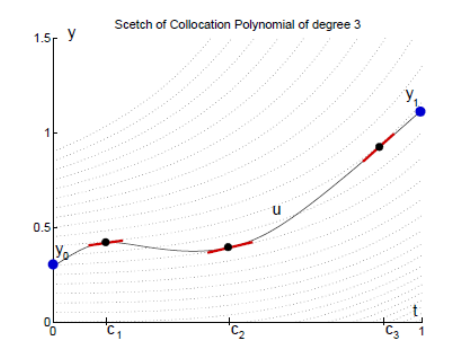
\includegraphics[width=.450\textwidth]{KolokazioMetodoa}
}
\caption{ \small kolokazio metodoak.}
\label{fig:kolokazio metodoak}
\end{figure}

\paragraph{\textbf{Adibidea}.} $s=1$  "Implicit Midpoint Rule" izeneko  $p=2$ ordeneko metodoa eta  $s=2$,  $p=4$ ordeneko metodoa.
\begin{equation*}
\begin{array}{c|c}
  \frac{1}{2} & \ \frac{1}{2} \\
  \hline
         & 1 \\
\end{array} \ \ \ ,  \ \ \ \ \ \ \ \ \
\begin{array}{c|c c}
  \frac{1}{2}-\frac{\sqrt{3}}{6} & \ \frac{1}{4} & \ \frac{1}{4}-\frac{\sqrt{3}}{6} \\
  \frac{1}{2}+\frac{\sqrt{3}}{6} & \ \frac{1}{4}+\frac{\sqrt{3}}{6} & \ \frac{1}{4} \\
  \hline
         &  \frac{1}{2} & \ \frac{1}{2} \\
\end{array}, \ \
\end{equation*}

Irudia 
 

\section{Konposizio metodoak.}

\subsection{Konposizio metodoak.}

Oinarrizko metodo baten konposizioaren bidez, orden handiagoko metodoak lortzen dira oinarrizko metodoaren propietateak mantenduz.

\paragraph*{\textbf{Definizioa orokorra}}.
$\phi_h$ oinarrizko metodoa eta $\gamma_1,\dots,\gamma_s$ zenbaki errealak emanik, urrats luzera hauen $\gamma_1 h,\gamma_2 h,\dots,\gamma_s h$ konposaketari dagokion konposizio metodoa,
\begin{equation}
\Psi_h=\phi_{\gamma_s h} \circ \dots \circ \phi_{\gamma_{1 h}}.
\end{equation}

\paragraph*{\textbf{Teorema}}.
Demagun $\phi_h$ urrats bakarreko eta $p$ ordeneko metodoa. Konposizio metodoa gutxienez $p+1$ ordeneko izango da baldin,
\[\gamma_1+\dots+\gamma_s=1\]
\begin{equation}
\gamma_1^{p+1}+\dots+\gamma_s^{p+1}=1
\end{equation}

\paragraph*{\textbf{Metodo simetrikoen konposizio simetrikoa}}.
$\phi_h$ metodoa $p=2$ ordenekoa eta simetrikoa izanik, era honetako konposizioak aurkitu dira,
\begin{equation}
\Psi_h=\phi_{\gamma_s h} \circ \phi_{\gamma_s-1 h} \circ \dots \circ \phi_{\gamma_{2 h}} \circ \phi_{\gamma_{1 h}} 
\end{equation}
non $\gamma_s=\gamma_1, \gamma_{s-1}=\gamma_2,\dots$ 

\paragraph*{\textbf{Algoritmoa}}.
Konposizio metodoen algoritmo orokorra honakoa izango litzateke:

\begin{algorithm}[H]
 \BlankLine
  \For{$n\leftarrow 1$ \KwTo $endstep$}
  {
   \BlankLine
    $Y_{0,n}=y_{n-1} $\;
    \BlankLine
   \For{i=1,2,...,s}
   {
    \BlankLine 
    $Y_{i,n}=\phi_{\gamma_i h}(Y_{i-1,n})$\;
   }
   \BlankLine
    $y_{n}=Y_{s,n}$\;
   \BlankLine
 }
 \caption{Konposizio metodoak.}
\end{algorithm}
 
\paragraph*{Oharrak}.
Algoritmoari buruzko hainbat ohar azpimarratuko ditugu:
\begin{enumerate}
\item{Esplizitua.}

Konposizio metodo hauek esplizituak dira. Metodo hauetan ez da ekuazio sistemarik askatu behar, eta kalkuluak azkarrak dira. 

\item{Sekuentziala.}
Urrats bakoitzaren kalkuluak modu sekuentzialean egin behar ditugu.

\item{Oinarrizko metodoa: Störmer-Verlet.}

Bigarren ordeneko ekuazio diferentzialak ditugunean, Störmer-Verlet integratzailean oinarritzen diren konposizio metodoekin
urrats bakoitzean $s$ ekuazio diferentzialaren balioztapena egin behar ditugu.

\end{enumerate}

\subsection{Gure inplementazioa.}

Gure erreferentzia, Stömer-Verlet metodoan oinarritzen den konposizio metodoa izango da. Zehazki, Sofroniok eta Spalettak ($2004$) aurkitutako $p=10$ ordeneko metodo optimoa. Beraz, lehenik Störmer-Verlet metodoa definituko dugu eta jarraian, metodoaren koefizienteak emango ditugu.   

\paragraph*{\textbf{Störmer-Verlet  metodoa}}.
$p=2$ ordeneko metodo sinplektikoa eta simetrikoa dugu.

\[p_{\frac{n+1}{2}}=p_n-\frac{h}{2} \triangledown_q H(p_{\frac{n+1}{2}},q_n) \]
\begin{equation}
q_{n+1}=q_n+\frac{h}{2} \big(\triangledown_p H(p_{\frac{n+1}{2}},q_n)+ \triangledown_p H(p_{\frac{n+1}{2}},q_{n+1}) \big)
\end{equation}
\[p_{n+1}=p_{\frac{n+1}{2}}-\frac{h}{2} \triangledown_q H(p_{\frac{n+1}{2}},q_{n+1}) \]

edo

\[q_{\frac{n+1}{2}}=q_n+\frac{h}{2} \triangledown_p H(p_n,q_{\frac{n+1}{2}}) \]
\begin{equation}
p_{n+1}=p_n-\frac{h}{2} \big(\triangledown_q H(p_n,q_{\frac{n+1}{2}})+ \triangledown_q H(p_{n+1},q_{\frac{n+1}{2}}) \big)
\end{equation}
\[q_{n+1}=q_{\frac{n+1}{2}}+\frac{h}{2} \triangledown_p H(p_{n+1},q_{\frac{n+1}{2}}) \]


\paragraph*{}Bigarren ordeneko ekuazio diferentziala ditugunean metodoa esplizitua da eta modu honetan labur daiteke,

\[p_{\frac{n+1}{2}}=p_n+\frac{h}{2} f(q_n)\]
\begin{equation}
q_{n+1}=q_n+h p_{\frac{n+1}{2}}
\end{equation}
\[p_{n+1}=p_{\frac{n+1}{2}}+\frac{h}{2}f(q_{n+1})\]

edo

\[q_{\frac{n+1}{2}}=q_n+\frac{h}{2} p_n\]
\begin{equation}
p_{n+1}=p_n-h f(q_{\frac{n+1}{2}})
\end{equation}
\[q_{n+1}=q_{\frac{n+1}{2}}+\frac{h}{2} p_{n+1}\]


\paragraph*{\textbf{10 ordeneko metodoa konposizio metodoa (CO1035)}}.
Sofronio eta Spalettaren ($2004$), $s=35$ eta $p=10$ ordeneko metodoa, orain arteko orden altuko konposizio metodo eraginkorrena kontsideratu daiteke.

\[\gamma_1=\gamma_{35}= 0.07879572252168641926390768\] 
\[\gamma_2=\gamma_{34}= 0.31309610341510852776481247\] 
\[\gamma_3=\gamma_{33}= 0.02791838323507806610952027\]
\[\gamma_4=\gamma_{32}= -0.22959284159390709415121340\] 
\[\gamma_5=\gamma_{31}= 0.13096206107716486317465686\] 
\[\gamma_6=\gamma_{30}= -0.26973340565451071434460973\] 
\[\gamma_7=\gamma_{29}= 0.07497334315589143566613711\] 
\[\gamma_8=\gamma_{28}= 0.11199342399981020488957508\] 
\[\gamma_9=\gamma_{27}= 0.36613344954622675119314812\] 
\[\gamma_{10}=\gamma_{26}= -0.39910563013603589787862981\] 
\[\gamma_{11}=\gamma_{25}= 0.10308739852747107731580277\]
\[\gamma_{12}=\gamma_{24}= 0.41143087395589023782070412\] 
\[\gamma_{13}=\gamma_{23}= -0.00486636058313526176219566\] 
\[\gamma_{14}=\gamma_{22}= -0.39203335370863990644808194\] 
\[\gamma_{15}=\gamma_{21}= 0.05194250296244964703718290\] 
\[\gamma_{16}=\gamma_{20}= 0.05066509075992449633587434\] 
\[\gamma_{17}=\gamma_{19}= 0.04967437063972987905456880\] 
\[\gamma_{18}= 0.04931773575959453791768001\]  


\section{Splitting metodoak.}

\subsection{Splitting metodoak.}

Demagun jatorrizko $\dot{\bf{y}}=\bf{f}(\bf{y})$ problema era honetan bana daitekeela,
\begin{equation}
\dot{\bf{y}}=\bf{f^{[1]}}(\bf{y})+\bf{f^{[2]}}(\bf{y})
\end{equation} 
non $\dot{\bf{y}}=\bf{f^{[1]}}(\bf{y})$ eta $\dot{\bf{y}}=\bf{f^{[2]}}(\bf{y})$ sistemen fluxu zehatzak, $\varphi_t^{[1]}$ eta $\varphi_t^{[2]}$ esplizituki kalkula daitezke. 

\paragraph*{\textbf{Lie-Trotter splitting}}.
$p=1$ ordeneko metodoak,
\[\phi_h^{*} = \varphi_h^{[2]} \circ \varphi_h^{[1]}\]
\begin{equation}
\phi_h = \varphi_h^{[1]} \circ \varphi_h^{[2]}
\end{equation}

\paragraph*{\textbf{Strang splitting}}.
$p=2$ ordeneko metodo simetrikoa,
\begin{equation}
\phi_h =  \varphi_{\frac{h}{2}}^{[1]} \circ \varphi_h^{[2]} \circ \varphi_{\frac{h}{2}}^{[1]}
\end{equation} 

\paragraph*{\textbf{Adibidea}}.
Störmer-Verlet metodoa, Strang Splitting metodoa dela ikusiko dugu. Suposatu dezagun Hamiltondar banagarria dugula, $H(p,q)=T(p)+U(q)$ . Jatorrizko sistema Hamiltondarra bitan banatuko dugu,

\begin{equation*}
\dot{p}=0 , \ \ \ \ \ \ \ \ \ \ \ \ \ \ \dot{p}=-U_q(q)
\end{equation*}
\begin{equation}
\dot{q}=T_p(p),\ \ \ \ \ \ \ \ \ \ \dot{q}=0  \ \ \ \ \ \ \ \
\end{equation}

eta integratuz lortuko ditugu bakoitzari dagokion ($\varphi_t^{[T]}$,$\varphi_t^{[U]}$) fluxu zehatzak,
\begin{equation*}
p(t)=p_0 , \ \ \ \ \ \ \ \ \ \ \ \ \ \ p(t)=p_0-t U_q(q_0)
\end{equation*}
\begin{equation}
q(t)=q_0+t T_p(p_0),\ \ \ \ \ \ \ \ \ \ q(t)=q_0  \ \ \ \ \ \ \ \
\end{equation}

Beraz, Störmer-Verlet metodoa bat dator Strang Splitting definizioarekin $\varphi_{\frac{h}{2}}^{[U]} \circ \varphi_h^{[T]} \circ \varphi_{\frac{h}{2}}^{[U]}$.

\paragraph*{\textbf{Splittig metodo orokorrak}}.
Konposizio metodoen modu berean, oinarrizko Splitting metodoak konposatuz orden altuagoko metodoak lortzen dira. $a_1,b_1,a_2,\dots,a_m,b_m$ koefiziente errealak izanik,

\begin{equation}
\Psi_h=\varphi^{[2]}_{b_m h} \circ \varphi^{[1]}_{a_m h} \circ \varphi^{[2]}_{b_m-1 h} \circ \dots \circ \varphi^{[1]}_{a_2 h} \circ \varphi^{[2]}_{b_1 h} \circ \varphi^{[1]}_{a_1 h}
\end{equation}

\begin{algorithm}[H]
 \BlankLine
  \For{$n\leftarrow 1$ \KwTo $endstep$}
  {
   \BlankLine
    $Y_{0,n}=y_{n-1} $\;
    \BlankLine
   \For{i=1,2,...,m}
   {
    \BlankLine 
    $Y_{i,n}=(\varphi^{[2]}_{b_i h} \circ \varphi^{[1]}_{a_i h})(Y_{i-1,n})$\ ;
   }
   \BlankLine
    $y_{n}=Y_{m,n}$\;
   \BlankLine
 }
 \caption{Splitting metodoak.}
\end{algorithm}


\subsection{Erreferentzia.}

N-gorputzeko problema grabitazionalaren Hamiltondarra $H(p,q)=T(p)+U(q)$, koordenatu sistema egokia erabiliz modu honetan $H=H_K+H_I$ ($|H_I|\ll|H_K|$) beridatzi daiteke. Azken egitura honetan oinarrituz orden altuko hainbat Spliiting metodo aurkitu dira. Gure errefentziazko metodoak Hamiltondar egitura honi bereziki egokitutako integratzaileak izango dira:

\begin{enumerate}
\item. $SABA_4$ (Laskar, 2001).

\paragraph*{Hamiltondarra}, $H=H_A+\epsilon H_B$ izanik eta goiko notazioa erabiliz,
\[SABA_4=\varphi^{[A]}_{c_1 h} \circ \varphi^{[B]}_{d_1 h} \circ \varphi^{[A]}_{c_2 h} \circ \varphi^{[B]}_{d_2 h}
         \circ  \varphi^{[A]}_{c_3 h}   \circ
          \varphi^{[B]}_{d_2 h} \circ \varphi^{[A]}_{c_2 h} \circ   \varphi^{[B]}_{d_1 h}\circ  \varphi^{[A]}_{c_1 h}
\]

\paragraph*{Koefizienteak},
\[c_1=\frac{1}{2}-\frac{\sqrt{525+70\sqrt{30}}}{70} , \ \ \ \ \ \ \ \ \ d_1=\frac{1}{4}-\frac{\sqrt{30}}{72}\]
\[c_2=\frac{\big( \sqrt{525+70 \sqrt{30}}-\sqrt{525-70 \sqrt{30}} \big)}{70} , \ \ \ \ \ \ \ \ \ d_2=\frac{1}{4}+\frac{\sqrt{30}}{72}\]
\[c_3=\frac{\sqrt{525-70\sqrt{30}}}{35} \ \ \ \ \ \ \ \ \ \ \ \ \ \ \ \ \]

\paragraph*{Corrected integrator}.
Urrats bat gehitutako integratzailea $SABAC_4$,
\[SABAC_4=\varphi{[B]}_\frac{-c}{2} \circ SABA_4 \circ \varphi{[B]}_\frac{-c}{2}\] 
non $c=0.003396775048208601331532157783492144$.\\

\item. $ABAH1064$ (Blanes, 2013).

\paragraph*{}Eguzki sistemaren integraziorako koordenatu Heliozentrikoei dagokion Hamiltondarra era honetakoa dugu,
\begin{equation*}
H(p,q)=H_K(p,q)+H_I(p,q), \ \ H_I(p,q)=T_1(p)+U_1(q) 
\end{equation*}

$H_I(p,q)$ fluxua zehazki kalkulatu ordez honen hurbilpen bat erabiliz,
\begin{equation*}
\varphi_t^I \approx \tilde{\varphi}_t^I= \varphi_{\frac{tb_i}{2}}^{[U_1]} \circ \varphi_tb_i^{[T_1]} \circ \varphi_{\frac{tb_i}{2}}^{[U_1]}
\end{equation*}

garatutako $ABAH1064$ Splitting metodoa aztertuko dugu,
\[ABAH1064=\prod\limits_{i=1}^{5} \varphi_{a_ih}^K \circ \tilde{\varphi}_{b_ih}^I\]

\[a_1=0.04731908697653382270404371796320813250988\]
\[a_2=0.2651105235748785159539480036185693201078\]
\[a_3=-0.009976522883811240843267468164812380613143\]
\[a_4=-0.05992919973494155126395247987729676004016\]
\[a_5=0.2574761120673404534492282264603316880356\]

\[b_1=0.1196884624585322035312864297489892143852\]
\[b_2=0.3752955855379374250420128537687503199451\]
\[b_3=-0.4684593418325993783650820409805381740605\]
\[b_4=0.3351397342755897010393098942949569049275\]
\[b_5=0.2766711191210800975049457263356834696055\]


\end{enumerate} 


\section{Kepler fluxua.}

\paragraph*{\textbf{Bi gorputzen problema}}. Kepler problemari dagokion Hamiltondarra,
\begin{equation}
H(\bf{p},\bf{q})=\frac{\mathbf{p}^2}{2m}-\frac{\mu}{\|\mathbf{q}\|}.
\end{equation}

Elkar erakartzen diren bi gorputzen mugimendua kalkulatzeko, gorputz baten kokapena koordenatu sistemaren jatorria kontsideratuko dugu. Honen arabera, $m=(1/m_1+1/m_2)^{-1}$ eta $\mu=Gm_1m2$ definituko ditugu. 


Hamiltondarrari dagozkion bigarren ordeneko ekuazio diferentzialak,

\begin{equation}
\ddot{\mathbf{q}}= - \frac{k\mathbf{q}}{\|\bf{q}\|^3} ,
\end{equation}
non $k= \mu / m$ eta  $\mathbf{q}\in \mathbb{R}^3$.


\paragraph*{\textbf{Ideia nagusia}}. Koordenatu kartesiarretatik koordenatu eliptikoetara $(a,e,i,\Omega,E)$ itzulpena egingo dugu. Kontutan hartuta $E$ (izena??) aldagai ezik beste aldagaiek konstante mantentzen direla, $E_0$ abiapuntua harturik, $\triangle t$ denbora tartea aurrera egingo dugu $E_1$ balioa berria kalkulatzeko. Azkenik, koordenatu eliptikoetatik koordenatu kartesiarrak berreskuratuko ditugu kokapen eta abiadura berriekin. 

\begin{equation*}
(\bf{q_0},\bf{v_0}) \in \mathbb{R}^6 \ \ \ \longrightarrow \ \ \  (a,e,i,\Omega,E_0) \in \mathbb{R}^6 
\end{equation*}

\begin{equation*}
\downarrow \triangle t
\end{equation*}

\begin{equation*}
(\bf{q_1},\bf{v_1}) \in \mathbb{R}^6 \ \ \ \longleftarrow \ \ \  (a,e,i,\Omega,E_1) \in \mathbb{R}^6 
\end{equation*}

\paragraph*{\textbf{Newton metodoa}}. Kepler-en ekuazioan oinarrituz ($E-e\sin E=n (t-t_p)$),  $E_1=\triangle E+E_0$ balioa kalkulatuko Newtonen metodoa aplikatuz,

\begin{equation*}
f(\triangle E)=\triangle E - ce \sin(\triangle E)- se (\cos(\triangle E)-1)-n \triangle t=0
\end{equation*}
\begin{equation}
\triangle E^{[k+1]}=\triangle E^{[k]}- \frac{f(\triangle E^{[k]})}{f'(\triangle E^{[k]})}
\end{equation}

\paragraph*{\textbf{Ekuazioak}}. Gure inplementazioan erabilitako ekuazio guztien azalpenak eta definizoak eranskinean eman ditugu.

\section{Laburpena.}

Hauek dira Eguzki sistemaren integraziorako konparatuko ditugun metodoak,

\begin{table}{htb}
\caption{Integrazio metodoen laburpena}
\label{tab:1}       % Give a unique label
\begin{tabular}{ c|c c c } 
           &  C1035             &  ABAH1064           & GAUSS-12           \\
 \hline
 	       & Konposizio met.    & Splitting met.     & IRK met.            \\
 	       & Sofronio (2004)    & Blanes et al. 2013 &                     \\
 \hline 
               &                    &                    &                 \\
 Hamiltoniarra & Orokorra           & Perturbatua        & Orokorra        \\ 	    
 Mota          & Esplizitua         & Esplizitua         & Inplizitua      \\ 
 Ordena        & 10                 & 10                 & 12              \\ 
 Atalak        & 35                 & 9                  & 6               \\ 
 Parall.       & Ez                 & Ez                 & Bai             \\  
\end{tabular}
\end{table}
 
